% =====================================================================
%  Trabalho de Probabilidade — Aplicações da Lei dos Grandes Números
%  Compilar com pdfLaTeX (recomendado: Overleaf). Codificação UTF-8.
% =====================================================================
\documentclass[12pt,a4paper]{article}

\usepackage[utf8]{inputenc}
\usepackage[T1]{fontenc}
\usepackage[brazil]{babel}
\usepackage{lmodern}
\usepackage{amsmath,amssymb,amsthm}
\usepackage{graphicx}
\usepackage{float}
\usepackage{booktabs}
\usepackage{caption}
\usepackage{geometry}
\usepackage{indentfirst}
\usepackage{microtype}
\usepackage{siunitx}
\usepackage[colorlinks=true,linkcolor=black,citecolor=black,urlcolor=blue]{hyperref}

\geometry{margin=2.5cm}
\graphicspath{{figuras/}}
\captionsetup{font=small,labelfont=bf}
\setlength{\parindent}{1.25em}
\setlength{\parskip}{0.25em}

% Operadores
\newcommand{\E}{\mathbb{E}}
\newcommand{\Prob}{\mathbb{P}}
\newcommand{\Var}{\operatorname{Var}}
\newcommand{\EP}{\operatorname{EP}}
\newcommand{\CV}{\operatorname{CV}}

% =====================================================================
\title{\textbf{Aplicações da Lei dos Grandes Números:\\
um estudo comparativo entre um fenômeno discreto e um contínuo}}

\author{%
  Júlio Neto \quad Victor Couto \quad Miguel Figueiredo \\
  \small Disciplina de Probabilidade --- Curso \\
  \small Instituição de Ensino
}
\date{\today}

% =====================================================================
\begin{document}

\maketitle

\begin{abstract}
\noindent
Este trabalho ilustra empiricamente a Lei dos Grandes Números (LGN) por meio de dois
conjuntos de dados de naturezas opostas: os sorteios da Mega-Sena (fenômeno
\emph{discreto}, com probabilidades conhecidas \emph{a priori}) e os retornos diários
de uma ação negociada na bolsa (fenômeno \emph{contínuo}, com média populacional
\emph{estimada} dos próprios dados). Mostra-se que a frequência relativa de um evento
converge para sua probabilidade teórica e que a média amostral converge para a
esperança, em ambos os casos. O argumento central é o contraste de \emph{velocidade}:
embora a LGN seja universal, o ritmo da convergência é governado pelo coeficiente de
variação $\CV=\sigma/|\mu|$, via erro relativo $\CV/\sqrt{n}$. Enquanto a loteria
($\CV\approx 0{,}57$) converge em poucas dezenas de observações, os retornos
($\CV\approx 18$) exigiriam mais de um século de dados para a mesma precisão.
Discute-se ainda a hipótese de independência e a transição natural da LGN para o
Teorema Central do Limite.
\end{abstract}

% =====================================================================
\section{Introdução}

A Lei dos Grandes Números (LGN) é um dos pilares da teoria da probabilidade. Em termos
intuitivos, ela formaliza a ideia de que, ao repetir um experimento aleatório muitas
vezes, a \emph{média} dos resultados observados se aproxima do valor \emph{esperado}, e
a \emph{frequência relativa} de um evento se aproxima de sua \emph{probabilidade}. É a
ponte rigorosa entre o conceito abstrato de probabilidade e aquilo que efetivamente
medimos no mundo.

O objetivo deste trabalho é \emph{demonstrar visualmente}, com dados reais, as duas
faces dessa lei e --- sobretudo --- evidenciar que a sua \emph{velocidade} de
convergência depende fortemente da variabilidade dos dados. Para isso, escolhemos dois
conjuntos deliberadamente contrastantes:

\begin{itemize}
  \item \textbf{Caso discreto:} o histórico de sorteios da \textbf{Mega-Sena}, em que
        as probabilidades são conhecidas por construção ($p = 6/60 = 0{,}10$ para uma
        dezena fixa; média $\mu = 30{,}5$ por dezena);
  \item \textbf{Caso contínuo:} os \textbf{retornos diários} de uma ação, em que a
        média populacional é minúscula frente a uma volatilidade muito alta e precisa
        ser \emph{estimada} dos dados.
\end{itemize}

A comparação entre os dois mostra que a LGN \emph{vale nos dois casos}
(universalidade), mas que a rapidez é radicalmente diferente --- um ponto que conduz
naturalmente ao Teorema Central do Limite (TCL).

% =====================================================================
\section{Fundamentação teórica}

\subsection{Esperança, variância e média amostral}

Seja $X_1, X_2, \dots, X_n$ uma sequência de variáveis aleatórias independentes e
identicamente distribuídas (i.i.d.), com esperança e variância finitas,
$\E[X_i] = \mu$ e $\Var(X_i) = \sigma^2 < \infty$. A \emph{média amostral} após $n$
observações é
\begin{equation}
  \bar{X}_n = \frac{1}{n}\sum_{i=1}^{n} X_i .
\end{equation}

\subsection{As duas formas da Lei dos Grandes Números}

\textbf{Lei Fraca} (convergência \emph{em probabilidade}): para todo $\varepsilon > 0$,
\begin{equation}
  \lim_{n\to\infty} \Prob\!\big(\,|\bar{X}_n - \mu| > \varepsilon\,\big) = 0 .
\end{equation}

\textbf{Lei Forte} (convergência \emph{quase certa}, mais forte):
\begin{equation}
  \Prob\!\Big(\lim_{n\to\infty} \bar{X}_n = \mu\Big) = 1 .
\end{equation}

Ambas afirmam que a média amostral se aproxima arbitrariamente de $\mu$ conforme $n$
cresce.

\subsection{A velocidade da convergência}

A média amostral é um estimador não-viesado de $\mu$, e sua variância \emph{encolhe}
com $n$:
\begin{equation}
  \E[\bar{X}_n] = \mu, \qquad
  \Var(\bar{X}_n) = \frac{\sigma^2}{n}
  \quad\Longrightarrow\quad
  \EP(\bar{X}_n) = \frac{\sigma}{\sqrt{n}} .
\end{equation}
Esse \emph{erro padrão} $\sigma/\sqrt{n}$ é o conceito-chave do trabalho. Para comparar
fenômenos de escalas diferentes, é útil o \emph{erro relativo}
\begin{equation}\label{eq:errorel}
  \frac{\EP(\bar{X}_n)}{|\mu|} = \frac{\sigma/\sqrt{n}}{|\mu|} = \frac{\CV}{\sqrt{n}},
  \qquad \CV = \frac{\sigma}{|\mu|},
\end{equation}
em que $\CV$ é o \emph{coeficiente de variação}. Invertendo a
Equação~\eqref{eq:errorel}, o número de observações necessário para um erro relativo
$e$ é
\begin{equation}\label{eq:custon}
  n = \left(\frac{\CV}{e}\right)^2 .
\end{equation}
A dependência quadrática implica que \emph{ganhar um dígito de precisão} ($10\times$
menor erro) custa $100\times$ mais dados.

\subsection{Frequência relativa como caso particular}

Para um evento $A$, defina a variável indicadora $X_i = \mathbf{1}\{A\text{ ocorre no
ensaio }i\}$, de modo que $X_i \sim \text{Bernoulli}(p)$ com $\E[X_i] = p = \Prob(A)$.
A média amostral coincide então com a frequência relativa:
\begin{equation}
  \bar{X}_n = \frac{N_A}{n} \;\xrightarrow{\;\Prob\;}\; p \quad (n\to\infty),
  \qquad N_A = \text{nº de ocorrências de } A .
\end{equation}
Ou seja, \emph{frequência relativa convergir para probabilidade} nada mais é do que a
LGN aplicada a indicadores de Bernoulli.

\subsection{Do limite ao formato: o Teorema Central do Limite}

A LGN diz \emph{para onde} a média converge; o Teorema Central do Limite (TCL) diz
\emph{com que forma}. Sob as mesmas hipóteses,
\begin{equation}\label{eq:tcl}
  Z_n = \frac{\bar{X}_n - \mu}{\sigma/\sqrt{n}}
  \;\xrightarrow{\;d\;}\; \mathcal{N}(0,1) \qquad (n\to\infty),
\end{equation}
isto é, $\bar{X}_n \approx \mathcal{N}(\mu,\,\sigma^2/n)$, \emph{qualquer que seja} a
distribuição de origem.

% =====================================================================
\section{Dados e metodologia}

\subsection{Conjuntos de dados}

\textbf{Mega-Sena.} Histórico de \num{2278} sorteios (de 1996 a 2018). Cada concurso
sorteia 6 dezenas distintas entre 1 e 60, totalizando \num{13668} dezenas. Os alvos
teóricos são conhecidos: $\Prob(\text{dezena fixa})=\binom{59}{5}/\binom{60}{6}=0{,}10$;
frequência de cada número $=1/60\approx0{,}0167$; e esperança por dezena $\mu=30{,}5$,
com variância da uniforme discreta $\sigma^2=(60^2-1)/12\approx299{,}9$
($\sigma\approx17{,}32$).

\textbf{Retornos financeiros.} Série de \num{2490} retornos diários da ação
\texttt{PETR4.SA} (2016--2026), obtida via biblioteca \texttt{yfinance} a partir do
preço de fechamento ajustado $P_t$. Calculou-se o retorno simples
$R_t = P_t/P_{t-1}-1$ (e, alternativamente, o logarítmico $r_t=\ln(P_t/P_{t-1})$).
Aqui a média populacional é \emph{estimada} da própria série.

\subsection{Ambiente computacional}

A análise foi conduzida em Python (\texttt{pandas}, \texttt{numpy},
\texttt{matplotlib}) sobre um ambiente Docker reproduzível com JupyterLab. Os
resultados estão organizados em três \emph{notebooks}: caso discreto, caso contínuo e
síntese. Todas as figuras deste documento foram geradas por esses \emph{notebooks}.

% =====================================================================
\section{Caso discreto: Mega-Sena}

\subsection{Frequência relativa \texorpdfstring{$\to$}{->} probabilidade}

Fixada uma dezena $k$, definimos por sorteio a indicadora
$X_i=\mathbf{1}\{\text{o sorteio }i\text{ contém }k\}\sim\text{Bernoulli}(0{,}10)$ e
acompanhamos a frequência relativa acumulada $\hat{p}_n$. A
Figura~\ref{fig:demoA} mostra o resultado para $k=10$.

\begin{figure}[H]
  \centering
  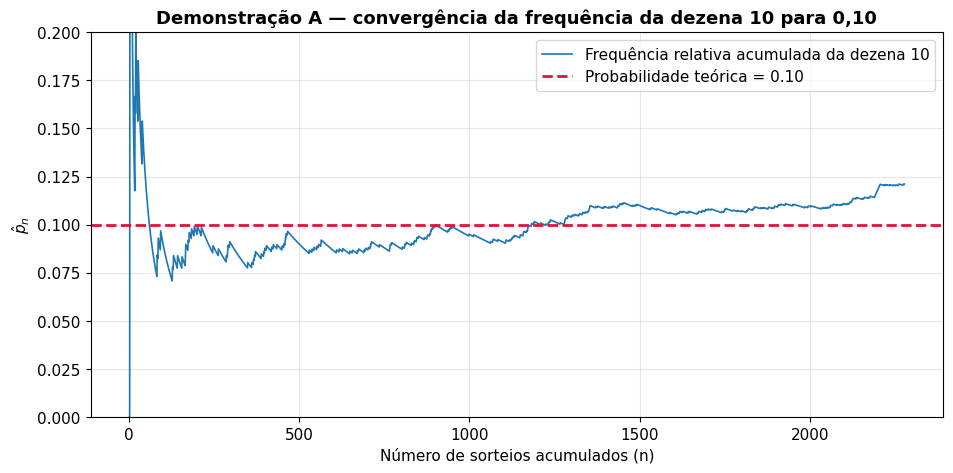
\includegraphics[width=0.8\textwidth]{megasena_demoA_dezena}
  \caption{Frequência relativa acumulada da dezena 10 convergindo para a
  probabilidade teórica $0{,}10$. As oscilações iniciais (entre $0$ e $0{,}2$) se
  amortecem conforme $n$ cresce.}
  \label{fig:demoA}
\end{figure}

As oscilações se amortecem à medida que $n$ aumenta --- a assinatura visual da LGN.
Vale uma observação de honestidade analítica: a curva termina em $\hat{p}_{2278}\approx
0{,}121$, e não exatamente em $0{,}10$. Isso \emph{não} contradiz a LGN: o erro padrão
de $\hat{p}_n$ é $\sqrt{p(1-p)/n}\approx0{,}0063$, de modo que o desvio observado
equivale a cerca de $3{,}4$ erros padrão. De fato, a dezena 10 está \emph{entre as mais
sorteadas} do período (empatada com a dezena 5, ambas com \num{276} aparições em
\num{2278} sorteios) --- ou seja, recaímos em um dos casos ``mais difíceis'' e, ainda
assim, a frequência ficou na casa de $0{,}12$. A lição é que \num{2278} ensaios ainda é pouco para um evento de
$p=0{,}10$, e que é o \emph{afunilamento} das oscilações (não a igualdade exata) que
evidencia a convergência.

A Figura~\ref{fig:demoAvarias} confirma que o fenômeno não depende da dezena escolhida:
diferentes números convergem todos para a mesma reta $0{,}10$.

\begin{figure}[H]
  \centering
  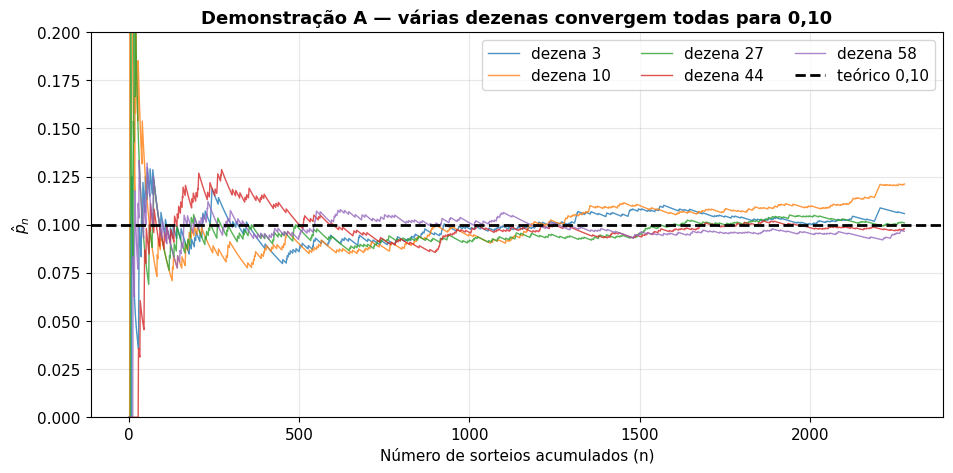
\includegraphics[width=0.8\textwidth]{megasena_demoA_varias}
  \caption{Várias dezenas: todas as frequências relativas acumuladas convergem para
  $0{,}10$, ilustrando que o resultado independe do número escolhido.}
  \label{fig:demoAvarias}
\end{figure}

Olhando o resultado \emph{final} (Figura~\ref{fig:barras}), a frequência relativa de
cada um dos 60 números, calculada sobre as \num{13668} dezenas, oscila em torno de
$1/60$ sem viés sistemático (todas entre $0{,}013$ e $0{,}020$). As diferenças são
flutuação amostral, coerente com um sorteio justo.

\begin{figure}[H]
  \centering
  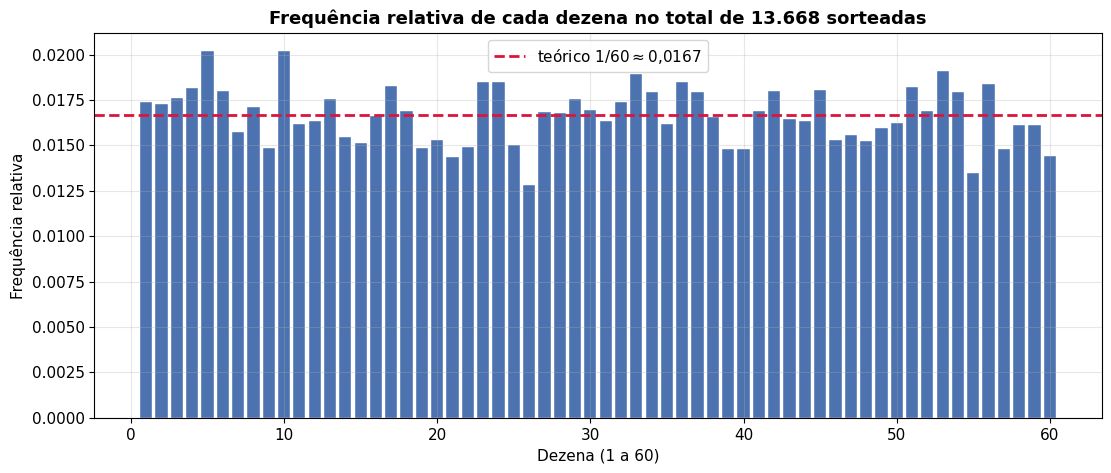
\includegraphics[width=0.95\textwidth]{megasena_freq_barras}
  \caption{Frequência relativa de cada dezena no total de \num{13668} sorteadas. As
  barras oscilam em torno da reta teórica $1/60\approx0{,}0167$.}
  \label{fig:barras}
\end{figure}

\subsection{Média amostral \texorpdfstring{$\to$}{->} esperança}

Tratando as \num{13668} dezenas (na ordem dos concursos) como observações, a média
acumulada converge para $\mu=30{,}5$ (Figura~\ref{fig:demoB}), terminando em
$\approx30{,}22$.

\begin{figure}[H]
  \centering
  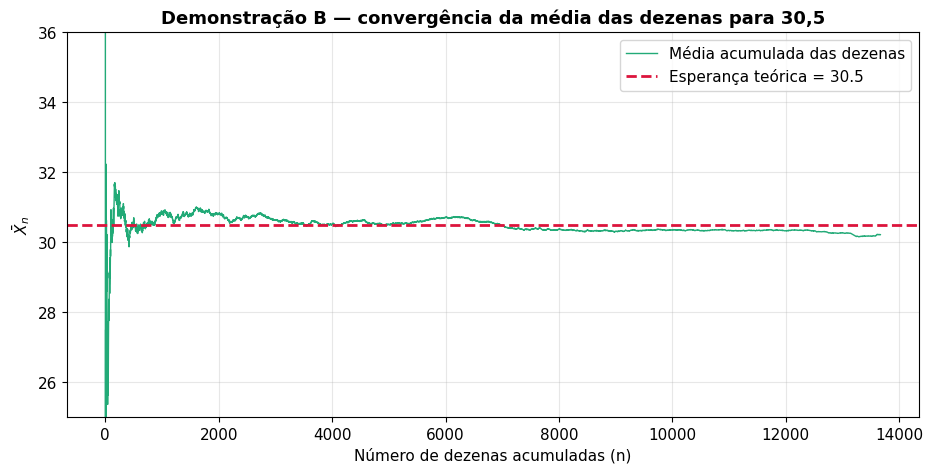
\includegraphics[width=0.8\textwidth]{megasena_demoB_media}
  \caption{Média acumulada das dezenas convergindo para a esperança teórica $30{,}5$.}
  \label{fig:demoB}
\end{figure}

Sobrepondo a faixa teórica $\mu\pm2\sigma/\sqrt{n}$ (Figura~\ref{fig:demoBfaixa}),
observa-se que a média empírica entra rapidamente no ``funil'' e ali permanece,
confirmando o decaimento do erro na taxa $\sigma/\sqrt{n}$.

\begin{figure}[H]
  \centering
  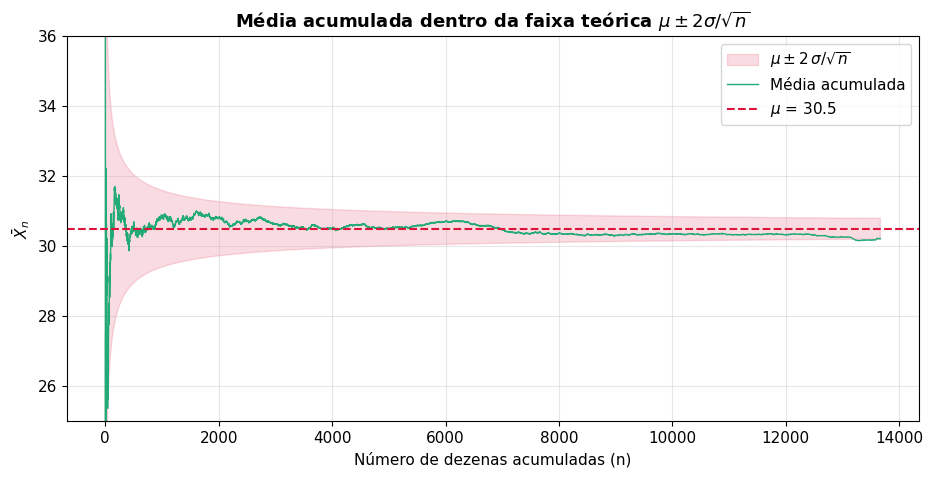
\includegraphics[width=0.8\textwidth]{megasena_demoB_faixa}
  \caption{Média acumulada dentro da faixa teórica $\mu\pm2\sigma/\sqrt{n}$, que
  afunila como $1/\sqrt{n}$.}
  \label{fig:demoBfaixa}
\end{figure}

% =====================================================================
\section{Caso contínuo: retornos financeiros}

\subsection{A natureza dos dados}

A Figura~\ref{fig:serie} mostra a série de retornos diários. A média (linha vermelha) é
praticamente indistinguível de zero diante da amplitude das oscilações --- imagem
direta de ``sinal minúsculo, ruído enorme''. Nota-se ainda o \emph{agrupamento de
volatilidade}: períodos turbulentos seguidos de períodos turbulentos.

\begin{figure}[H]
  \centering
  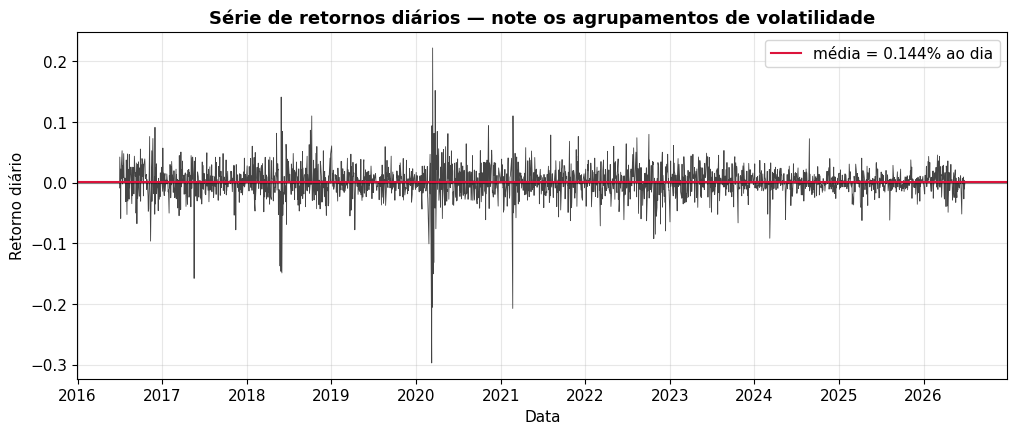
\includegraphics[width=0.95\textwidth]{retornos_serie}
  \caption{Série de retornos diários. A média é quase nula frente à volatilidade, e a
  turbulência ocorre em ondas (\emph{volatility clustering}).}
  \label{fig:serie}
\end{figure}

As estatísticas-resumo confirmam o quadro: média
$\hat{\mu}\approx0{,}001445$ ($0{,}14\%$ ao dia), desvio
$\sigma\approx0{,}0259$ ($2{,}59\%$ ao dia), e portanto
$\CV=\sigma/|\hat\mu|\approx17{,}9$. Pela Equação~\eqref{eq:custon}, atingir um erro
relativo de $10\%$ exigiria $n\approx\num{32070}$ pregões --- cerca de \textbf{127
anos}.

\subsection{Convergência lenta e ruidosa}

A média acumulada (Figura~\ref{fig:mediaacum}) passa anos longe do alvo, inclusive
negativa por longos trechos, aproximando-se de $\hat\mu$ apenas perto do fim. O ponto
final coincide com $\hat\mu$ por construção (o alvo é a média de toda a série); o que
demonstra a LGN é o \emph{caminho}, não o ponto final.

\begin{figure}[H]
  \centering
  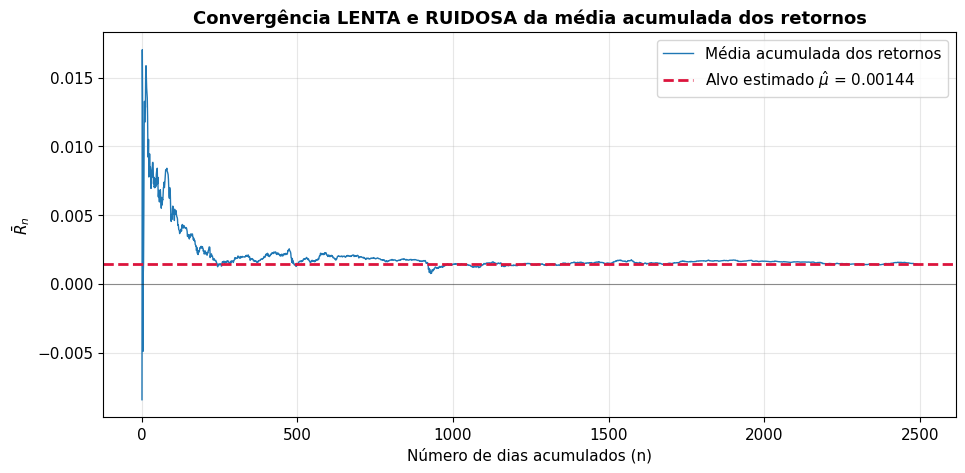
\includegraphics[width=0.8\textwidth]{retornos_media_acum}
  \caption{Média acumulada dos retornos: convergência lenta e ruidosa para a média
  estimada $\hat\mu$, em forte contraste com a loteria.}
  \label{fig:mediaacum}
\end{figure}

A faixa teórica (Figura~\ref{fig:retfaixa}) é larguíssima e afunila devagar: mesmo ao
fim de uma década, ela ainda \emph{inclui o zero}. Em termos práticos, com $\sim$10 anos
de dados não conseguimos afirmar com segurança que a média diária difere de zero.

\begin{figure}[H]
  \centering
  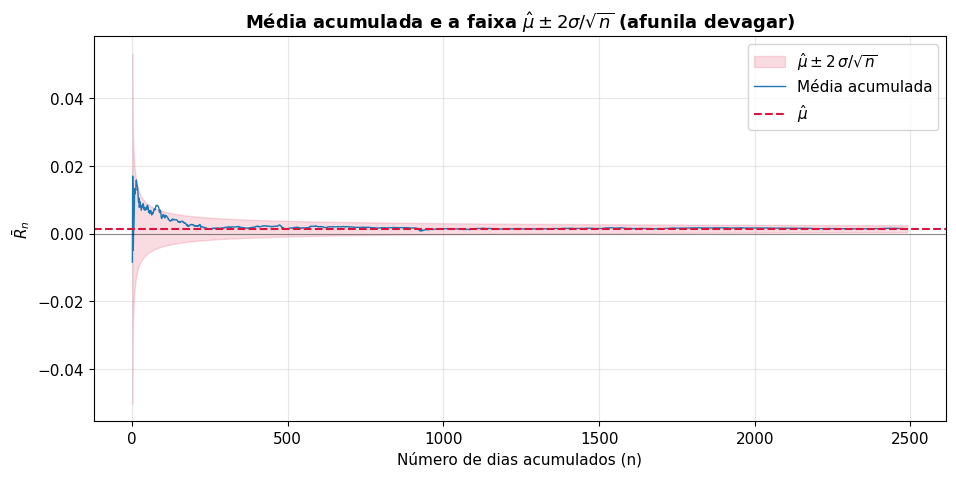
\includegraphics[width=0.8\textwidth]{retornos_faixa}
  \caption{Média acumulada e faixa $\hat\mu\pm2\sigma/\sqrt{n}$. Por causa do $\sigma$
  elevado, a faixa permanece larga e contém o zero ao fim da série.}
  \label{fig:retfaixa}
\end{figure}

\subsection{A variância da média encolhe como \texorpdfstring{$\sigma^2/n$}{sigma2/n}}

Um experimento de reamostragem (\emph{bootstrap}) confirma
$\Var(\bar{R}_n)=\sigma^2/n$. Para tamanhos crescentes $n$, a distribuição das médias
amostrais se concentra em torno de $\hat\mu$ (Figura~\ref{fig:reamostragem}). A
Tabela~\ref{tab:reamostragem} mostra que o desvio empírico das médias coincide com o
$\sigma/\sqrt{n}$ teórico.

\begin{figure}[H]
  \centering
  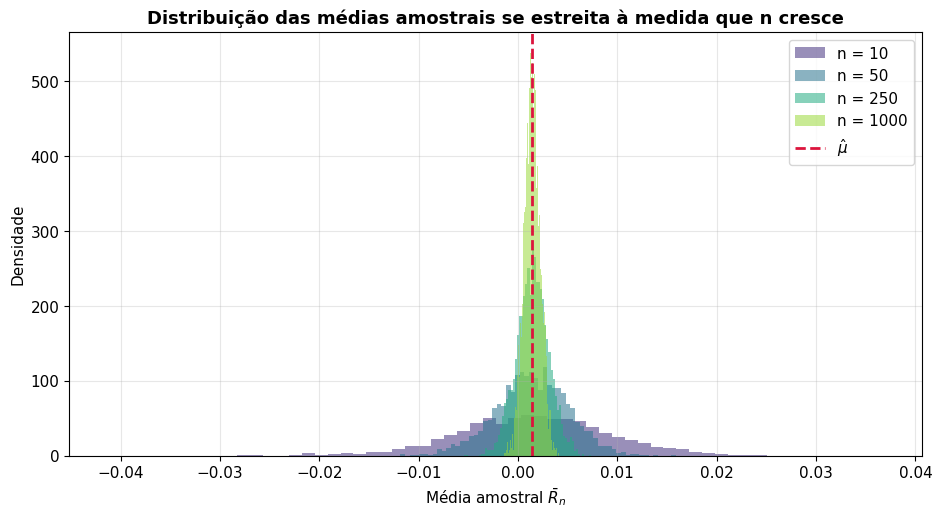
\includegraphics[width=0.8\textwidth]{retornos_reamostragem}
  \caption{Distribuição das médias amostrais para $n$ crescente: mais altas e estreitas
  conforme $n$ aumenta, todas centradas em $\hat\mu$.}
  \label{fig:reamostragem}
\end{figure}

\begin{table}[H]
  \centering
  \caption{Desvio das médias amostrais (\emph{bootstrap}, \num{3000} amostras) versus
  previsão teórica $\sigma/\sqrt{n}$.}
  \label{tab:reamostragem}
  \begin{tabular}{rcc}
    \toprule
    $n$ & desvio empírico & $\sigma/\sqrt{n}$ teórico \\
    \midrule
    10   & 0,008237 & 0,008181 \\
    50   & 0,003725 & 0,003659 \\
    250  & 0,001638 & 0,001636 \\
    1000 & 0,000819 & 0,000818 \\
    \bottomrule
  \end{tabular}
\end{table}

% =====================================================================
\section{Síntese e ponte para o Teorema Central do Limite}

\subsection{As duas convergências no mesmo eixo}

Em escala log-log, o erro relativo $|\bar{X}_n-\mu|/|\mu|$ dos dois casos decai com a
\emph{mesma} inclinação $-\tfrac12$ (a assinatura do $1/\sqrt{n}$), separado apenas
pela \emph{altura} --- justamente a razão entre os coeficientes de variação
(Figura~\ref{fig:loglog}).

\begin{figure}[H]
  \centering
  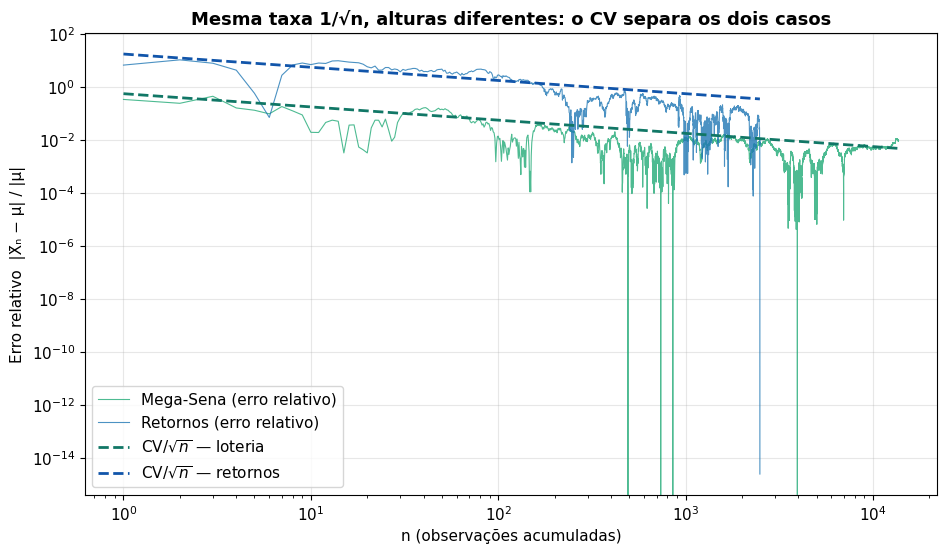
\includegraphics[width=0.85\textwidth]{sintese_loglog}
  \caption{Erro relativo da média acumulada para os dois casos, em escala log-log. As
  curvas têm a mesma taxa $1/\sqrt{n}$; o coeficiente de variação determina a altura.}
  \label{fig:loglog}
\end{figure}

A Tabela~\ref{tab:custo} traduz isso em custo de dados (Equação~\eqref{eq:custon}).

\begin{table}[H]
  \centering
  \caption{Número de observações para um dado erro relativo, por
  Equação~\eqref{eq:custon}.}
  \label{tab:custo}
  \begin{tabular}{lccc}
    \toprule
    Erro relativo & Mega-Sena ($n$) & Retornos ($n$) & Retornos ($\sim$anos) \\
    \midrule
    10\,\% & 32     & \num{32070}   & 127     \\
    5\,\%  & 129    & \num{128280}  & 509     \\
    1\,\%  & 3224   & \num{3207000} & \num{12726} \\
    \bottomrule
  \end{tabular}
\end{table}

\subsection{Da LGN ao TCL}

Padronizando as médias amostrais conforme a Equação~\eqref{eq:tcl}, verifica-se a
emergência da normal mesmo quando os dados de origem não são normais. Na loteria
(distribuição uniforme), a aproximação é \emph{rápida}: já em $n\approx5$--$30$ o
histograma coincide com a normal-padrão (Figura~\ref{fig:tclloteria}).

\begin{figure}[H]
  \centering
  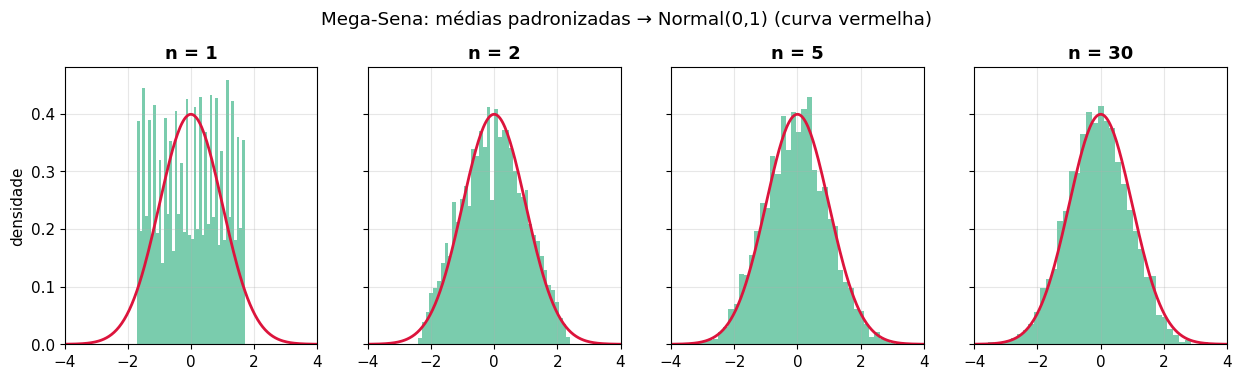
\includegraphics[width=\textwidth]{tcl_loteria}
  \caption{Mega-Sena: médias padronizadas convergindo para $\mathcal{N}(0,1)$ (curva
  vermelha). Partindo de uma uniforme, a forma de sino surge já com poucos termos.}
  \label{fig:tclloteria}
\end{figure}

Nos retornos (caudas pesadas), a aproximação é \emph{mais lenta}: para $n$ pequeno o
histograma é pontiagudo e de caudas grossas, e a normal só se firma por volta de
$n=250$ (Figura~\ref{fig:tclretornos}).

\begin{figure}[H]
  \centering
  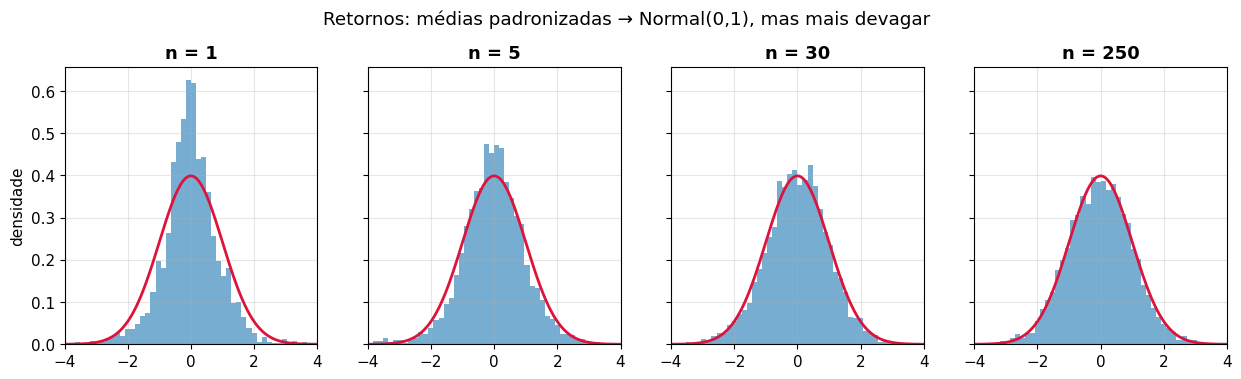
\includegraphics[width=\textwidth]{tcl_retornos}
  \caption{Retornos: médias padronizadas convergindo para $\mathcal{N}(0,1)$, porém
  mais devagar, devido às caudas pesadas da distribuição de origem.}
  \label{fig:tclretornos}
\end{figure}

A mesma mensagem da LGN reaparece no TCL: a convergência ocorre nos dois casos
(universalidade), mas é mais lenta onde a variabilidade é maior.

% =====================================================================
\section{Discussão crítica}

\paragraph{Alvo conhecido vs.\ estimado.} Na loteria, comparamos as curvas com valores
\emph{deduzidos} ($0{,}10$; $1/60$; $30{,}5$), o que torna o caso um laboratório ideal.
Nos retornos, o alvo $\mu$ é \emph{estimado} da própria série --- situação mais
realista, em que a incerteza sobre o próprio alvo se soma à da estimativa.

\paragraph{Hipótese i.i.d.} A LGN clássica supõe observações i.i.d. Os sorteios são
fisicamente independentes entre concursos (hipótese plausível); dentro de um mesmo
sorteio, contudo, as 6 dezenas são extraídas sem reposição, logo não são estritamente
independentes --- uma violação branda que não compromete o resultado. Já os retornos
financeiros apresentam \emph{dependência temporal} (agrupamento de volatilidade),
\emph{não-estacionariedade} e \emph{caudas pesadas}. A aplicação da LGN/TCL nesse caso é
uma \emph{aproximação informada}, amparada por versões mais fracas dessas leis (para
processos estacionários e ergódicos): a convergência ocorre, apenas mais devagar.

\paragraph{Lei fraca vs.\ forte.} O que enxergamos nos gráficos --- uma trajetória que
se aproxima de $\mu$ e ali permanece --- é a intuição da Lei Forte (convergência quase
certa). A Lei Fraca faz uma afirmação sobre a probabilidade de desvio para cada $n$
fixo. Para fins de visualização, ambas indicam o mesmo: a média converge.

% =====================================================================
\section{Conclusão}

A partir de dois conjuntos de dados reais e de naturezas opostas, verificamos
empiricamente as duas faces da Lei dos Grandes Números: a frequência relativa converge
para a probabilidade (caso particular com indicadores de Bernoulli) e a média amostral
converge para a esperança. As principais conclusões são:

\begin{enumerate}
  \item \textbf{Universalidade.} A LGN (e o TCL) valem tanto para um sorteio discreto e
        simétrico quanto para retornos contínuos de cauda pesada; a validade não depende
        da forma da distribuição.
  \item \textbf{Velocidade.} O ritmo da convergência é governado pelo coeficiente de
        variação $\CV=\sigma/|\mu|$, via erro relativo $\CV/\sqrt{n}$. Com
        $\CV\approx0{,}57$, a loteria converge em dezenas de observações; com
        $\CV\approx18$, os retornos precisariam de cerca de \num{1000} vezes mais dados
        para a mesma precisão.
  \item \textbf{Custo da precisão.} Pela relação $n=(\CV/e)^2$, cada dígito adicional de
        precisão custa $100\times$ mais observações.
  \item \textbf{Honestidade sobre as hipóteses.} A aproximação i.i.d.\ é quase exata na
        loteria e apenas aproximada nos retornos, o que reforça a leitura cuidadosa dos
        resultados.
  \item \textbf{Da LGN ao TCL.} A LGN indica o destino da média; o TCL descreve a forma
        (normal) e a taxa da chegada. Juntos, explicam a centralidade das médias na
        estatística e por que algumas são muito mais difíceis de estimar que outras.
\end{enumerate}

Em uma única frase: \emph{a Lei dos Grandes Números é a mesma para todos os fenômenos;
o que muda é a velocidade com que ela se manifesta}.

% =====================================================================
\clearpage
\begin{thebibliography}{9}
\bibitem{yfinance} YFINANCE. \emph{Yahoo! Finance market data downloader}.
  Disponível em: \url{https://github.com/ranaroussi/yfinance}. Acesso em: 29 jun. 2026.
\bibitem{kaggle} BIZARRI, V. B. \emph{Sorteios Mega-Sena}. Kaggle. Disponível em:
  \url{https://www.kaggle.com/datasets/viniciusbbizarri/sorteiosmegasena}.
  Acesso em: 29 jun. 2026.
\end{thebibliography}

\end{document}
